\documentclass[11pt]{article}
\usepackage[toc,page]{appendix}
\usepackage{amsmath, amssymb}
\usepackage[style=apa,backend=biber]{biblatex}
%\usepackage{biblatex}
\addbibresource{references.bib}
\usepackage{graphicx}
\usepackage{tikz}
\usetikzlibrary{automata,positioning,shapes.geometric, arrows.meta, fit, backgrounds, calc, chains}
%\usepackage{kpfonts}
\usepackage{float}
\usepackage[margin=1in]{geometry}
\usepackage{cancel}
\usepackage{epsfig}
\usepackage{tikz-3dplot}
\usepackage{darkmode}
\usepackage{dirtytalk}
\usepackage{longtable,booktabs,array}
\usepackage{calc} % for calculating minipage widths
% Correct order of tables after \paragraph or \subparagraph
\usepackage{etoolbox}
\usepackage{hyperref}
\hypersetup{
    colorlinks=true,
    linkcolor=blue,
    filecolor=magenta,      
    urlcolor=cyan,
    pdftitle={Hermeneutic Calculator},
    citecolor=blue,
    }


\urlstyle{same}
%\usepackage{tocloft}

% Optional: define some custom colors
\definecolor{sliceRed}{RGB}{225,224,91} % matching "varyellow" from your code
\definecolor{linkYellow}{RGB}{255,215,0}  % a golden yellow
\tdplotsetmaincoords{70}{110}

\title{Multiplication Strategies: Doubling}
\author{Theodore M. Savich}


\begin{document}
\maketitle
\subsection*{Doubling}

\subsubsection*{Description of Strategy:}
\begin{itemize}
    \item \textbf{Objective:} Use doubling to quickly reach the total number of items by doubling group sizes or totals.
    \item \textbf{Method:} Double the number of items (and the number of groups) repeatedly until reaching or surpassing the target total, then adjust as needed.
\end{itemize}

\subsubsection*{Automaton Type:}
\textbf{Finite State Automaton with Registers (Counters):}  
Counters are used to track the current total and the number of groups.

\subsubsection*{Formal Description of the Automaton}

We define the automaton as the tuple
\[
M = (Q,\, \Sigma,\, \delta,\, q_{0/accept},\, F,\, V)
\]
where:
\begin{itemize}
    \item \( Q = \{q_{0/accept},\, q_{\text{double}},\, q_{\text{check}},\, q_{\text{adjust}}\} \) is the set of states. Here, \(q_{0/accept}\) serves as both the start and accept state.
    \item \(\Sigma\) is the input alphabet (used to initialize the problem parameters).
    \item \( F = \{q_{0/accept}\} \) is the set of accepting states.
    \item \( V = \{\text{CurrentTotal (CT)},\, \text{CurrentGroups (CG)},\, \text{GroupSize (S)},\, \text{TotalGroups (N)}\} \) is the set of registers.
\end{itemize}

The key transitions are as follows:
\begin{enumerate}
    \item \textbf{Initialization:} From \(q_{0/accept}\), on reading the input values (with \(S\) and \(N\)), initialize \(CT \gets S\) and \(CG \gets 1\), then transition to \(q_{\text{double}}\).
    \item \textbf{Doubling:} In \(q_{\text{double}}\), repeatedly double both \(CT\) and \(CG\) (i.e., update \(CT \gets 2 \times CT\) and \(CG \gets 2 \times CG\)) until \(CG \ge N\).
    \item \textbf{Checking:} In \(q_{\text{check}}\), if \(CG = N\) then the target total is reached, and the automaton transitions to the accept state. If \(CG > N\), transition to \(q_{\text{adjust}}\) to fine-tune \(CT\).
    \item \textbf{Adjustment:} In \(q_{\text{adjust}}\), adjust \(CT\) appropriately (e.g., subtract the excess) before outputting the final total.
\end{enumerate}

\subsubsection*{Automaton Diagram for Doubling}

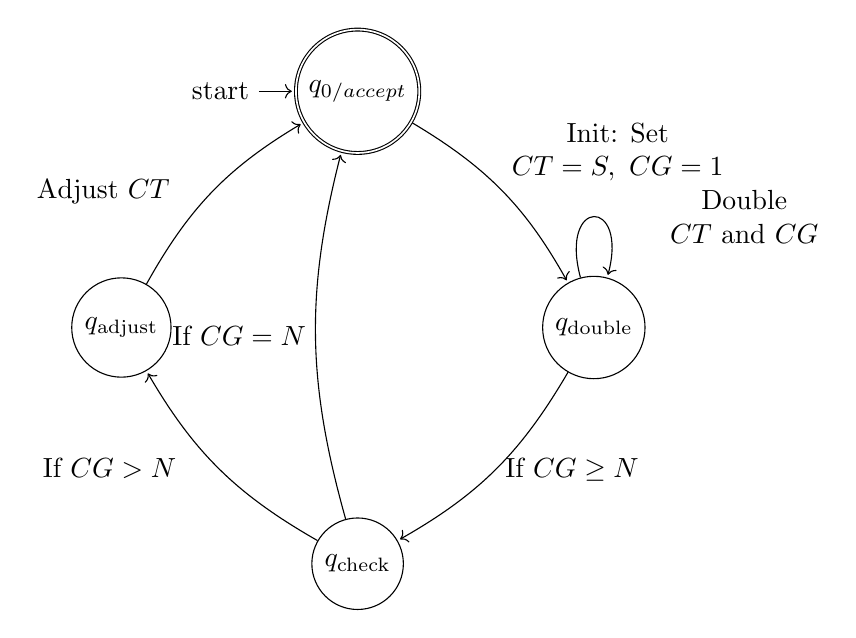
\begin{tikzpicture}[
    shorten >=1pt,
    auto,
    node distance=3cm,
    every state/.style={minimum size=1cm}
]
    % Arrange four states on a circle:
    % q_{0/accept} at 90°, q_{double} at 0°, q_{check} at 270°, q_{adjust} at 180°.
    \node[state, initial, accepting] (q0) at (90:3cm) {$q_{0/accept}$};
    \node[state] (q1) at (0:3cm) {$q_{\text{double}}$};
    \node[state] (q2) at (270:3cm) {$q_{\text{check}}$};
    \node[state] (q3) at (180:3cm) {$q_{\text{adjust}}$};

    \path[->]
        (q0) edge[bend left=15] node[above right, align=center] {Init: Set \\ \(CT=S,\ CG=1\)} (q1)
        (q1) edge[loop above] node[right=24pt, align=center] {Double \\ \(CT\) and \(CG\)} (q1)
        (q1) edge[bend left=15] node[right, align=center] {If \(CG \ge N\)} (q2)
        (q2) edge[bend left=15] node[left, align=center] {If \(CG=N\)} (q0)
        (q2) edge[bend left=15] node[left=12pt, align=center] {If \(CG>N\)} (q3)
        (q3) edge[bend left=15] node[left=12pt, align=center] {Adjust \(CT\)} (q0);
\end{tikzpicture}
\end{document}